% !TeX program = pdfLaTeX
\documentclass[12pt]{article}
\usepackage{amsmath}
\usepackage{graphicx,psfrag,epsf}
\usepackage{enumerate}
\usepackage{natbib}
\usepackage{textcomp}
\usepackage[hyphens]{url} % not crucial - just used below for the URL
\usepackage{hyperref}
\providecommand{\tightlist}{%
  \setlength{\itemsep}{0pt}\setlength{\parskip}{0pt}}

%\pdfminorversion=4
% NOTE: To produce blinded version, replace "0" with "1" below.
\newcommand{\blind}{0}

% DON'T change margins - should be 1 inch all around.
\addtolength{\oddsidemargin}{-.5in}%
\addtolength{\evensidemargin}{-.5in}%
\addtolength{\textwidth}{1in}%
\addtolength{\textheight}{1.3in}%
\addtolength{\topmargin}{-.8in}%

%% load any required packages here

\begin{document}

\def\spacingset#1{\renewcommand{\baselinestretch}%
{#1}\small\normalsize} \spacingset{1}

%%%%%%%%%%%%%%%%%%%%%%%%%%%%%%%%%%%%%%%%%%%%%%%%%%%%%%%%%%%%%%%%%%%%%%%%%%%%%%

\if0\blind
{
  \title{\bf Statistical Methods for Accounting Systems}

  \author{
        Stijn Masschelein \thanks{The authors are grateful for comments by seminar participants at
Australian National University, Leuven University, and the 2018 AFAANZ
conference.} \\
    University of Western Australia Business School\\
     and \\     Frank Moers \\
    Maastricht University School of Business and Economics\\
      }
  \maketitle
} \fi

\if1\blind
{
  \bigskip
  \bigskip
  \bigskip
  \begin{center}
    {\LARGE\bf Statistical Methods for Accounting Systems}
  \end{center}
  \medskip
} \fi

\bigskip
\begin{abstract}
Following the theoretical innovations of complementarity theory, management control studies have investigated potential interdependencies between management control practices. In this paper, we compare the two dominant statistical specifications in the management control literature to test for the presence of interdependencies. While prior literature focuses on the differences in the assumption of optimality between the demand specification and the performance specification, we make all ancillary assumptions explicit. Our stimulation results reveal that the demand specification is more robust to variations in optimality and the presence of correlated omitted variables than the performance specification. We use these results to formulate guidance for future research into interdependencies between management control practices.
\end{abstract}

\noindent%
{\it Keywords:} Complementarity Theory, Management Control, Statistical Methods
\vfill

\newpage

\spacingset{1.15}

\section{Introduction}\label{introduction}

 Complementarity theory posits that interdependent management control practices can be seen as one coherent management control system \citep{Milgrom1995, Grabner2013}. Different streams of literature have investigated such interdependencies between management control practices. For instance, agency theory argues that incentive design and delegation of decision rights are complements \citep{Holmstrom1994}. The management accounting literature has established that at least under certain conditions, delegation of more decision rights to managers complements incentive systems \citep{Moers2006, Indjejikian2012, Bouwens2007}. Drawing on the original work by Simons \citetext{\citeyear{Simons1995}; \citeyear{Simons2000}}, the levers of control literature has investigated potential complementarities between the four levers \citep{Widener2007}. Lastly, the budgeting literature has long argued that the effectiveness of budget participation depends on the the extent to which the budget is used to evaluate employees \citep{Brownell1991, Dunk1993}.
 
 \textbf{While the focus on interdependencies in the management control literature is relatively new, the literature has a longer tradition rooted in contingency theory of investigating the environmental factors that favor certain management control practices or certain combinations of practices (\citet{Grabner2013}). TODO: Add a couple of examples here and in the literature review. To be consistent with the current state of the management control literature, our theoretical model assumes that the effectiveness of individual management control practices depends on the environment and on other practices.}
 
 This paper compares the two main specifications to empirically test for an interdependency between two practices: the performance specification and the demand specification \citep{Grabner2013}.The demand approach assumes that firms simultaneously choose the optimal level of practices taking into account the interdependency and the firm's environment. Under this assumption, all firms adopt the best possible combination of practices for their environment and firms with different combinations of practices have the same performance. Furthermore, controlling for environmental factors, complementary practices are positively correlated with each other. The performance specification assumes that there are a sufficient number of firms that deviate from those optimal choices which allows researchers to detect performance differences. Under this assumption, the interaction between the two practices is positively correlated with performance \citep{Athey1998, Grabner2013}. The distinction between both specifications is similar to the distinction between contingency fit and congruence fit in the contingency literature \citep{VandeVen1985a, Gerdin2004}. 

\textbf{The current state of the literature treates the assumption of optimality as untestable, i.e.~authors have to make the case that it is either reasonable that the average observation has adopted the optimal management control system or that decision makers are still figuring out the optimal system \citep{Grabner2013}.}

\begin{quote}
Which {[}specification{]} to use is both a theoretical (assumption of agents as perfectly or boundedly rational) and an empirical (market imperfections, exogenous shocks, experimentation, etc) issue because the likelihood of finding evidence of the former depends on the latter and vice versa (Grabner and Moers, 2013; Gerdin and Greve, 2004). (in Johansson, 2016).
\end{quote}

\begin{quote}
decision makers may not have been sufficiently well informed such that they chose efficiency or output enhancing combinations of practices.
\citep{Carree2011}
\end{quote}

\textbf{Others have argued that the performance specification can be applied ``as long a the populaetion of organizations includes a reasonable number of organizations that takes non-optimal combinations of practice'' \citep{Carree2011}. TODO: I would be nice find more of these quotes because we show that this is a misconception.}

About the conditional correlation approach.
\begin{quote}
While this approach certainly has intuitive appeal and is easy to implement, it also relies on a strong assumption that the set of conditioning variables is reasonably complete. Without a well-specified reduced form regression, the correlation between the residual (p. 459) terms might not signal complementarity but rather the presence of a third factor that is correlated with the two organizational design choices under consideration. from (Hoffman and van Lent).
\end{quote}

\begin{quote}
This focus is appropriate as the control problems examined in this study (i.e. the alignment of behaviours to the strategic objectives of the firm) are complex and require significant experimentation by top management, particularly in conditions characterized by uncertainty such as the prospector strategic context (Simons, 1995). Hence it is unlikely that firms will be, on average, in an optimal equilibrium. in \citep{Bedford2016}
\end{quote}

We theoretically derive the demand and performance specification from the same unobserved performance function and show the potential statistical problems that arise with either approach. The demand specification is misspecified when the assumption of average optimal choices is not met. Further, this specification requires an additional assumption that the interdependency cannot be too strong. Finally, the estimation of the demand specification is vulnerable to simultaneity bias. The performance specification is potentially misspecified and has less power when the practices are closer to optimal.

\textbf{Lastly, we show how both specifications suffer from the same omitted correlated variable bias. An estimate of the interdependency between two practices is biased when the empirical specification does not control for an environmental factor (or third practice) on which both practices of interest depend and the decision makers adopt the optimal management control system. This result highlights the importance to consider contingency and interdependency effects at the same time when testing for complementarities between management control practices. While this problem is widely recognised for the demand specification \citep[\citet{Grabner2013}]{Arora1996}, there is a misconception in the methodological literature that the production specification does not suffer from this problem \citep{Carree2011}. In addition, we show how both specifications can control for the bias when all relevant environmental factors and practices are observed. Unfortunately, the most commonly used variant of the production specification does not address the bias properly.}

\textbf{Because the vulnerabilities of both specifications depend on the level of optimality, this study compares the robustness of both specifications to variations in the level of optimality in a simulation study.} The results show that the demand approach has appropriate type I error rates while maintaining power to detect a real complementary effect even at low levels of optimality. In contrast, the theoretically derived performance function approach suffers from elevated type I error rates and loses power to detect true interdependencies. In addition, we compare the performance specification as it is typically implemented in the literature to the theoretically derived performance function specification. The typical specification exhibits inflated type I error rates while having little power to detect a real interdependency at all but the lowest levels of optimality.

This study provides three recommendations for studies that explicitly or implicitly test for interdependencies between managerial choices. First of all, firms are not required to perfectly design the management control system to prefer the demand approach over the performance approach. When performance data is available, it is still advisable to estimate the demand functions before estimating the performance functions \citep{Aral2012, Cassiman2006}. Second, when prior theory and data indicates that the individual practices are contingent on environmental factors, studies should appropriately control for these factors. \textbf{Because the management control literature has a rich history of studying contingency effects, we believe most management control settings will warant appropriate controls for environmental factors.} In the demand specification, controlling for environmental factors means including the control variables as separate independent variables. In the performance specification, controlling for contingency effects requires including the interaction of the environmental factors with the management control practices. Of the 6 published studies using the performance specification approach following \citet{Grabner2013}, only \citet{Bedford2016} appropriately controls for contingency factors. Third, this study highlights the importance of carefully laying out the theoretical and statistical assumptions of a model \citep{Chenhall2007}. Studies on interdependencies in management accounting defend their statistical approach on grounds of the optimality of the management practices. The results of the simulation show that omitted correlated variables, such as environmental factors, should be as much a concern as the assumption of optimality.

The remainder of this paper is structured as follows. First, we derive the demand and performance specifications. Second, we compare the robustness of the different specifications in a simulation study. Last, we summarise the simulation results, provide further guidance for researchers who estimate interdependencies, and lay out how future research can address the problems with the specifications we investigate in this study.

\section{Model and formal analysis}\label{model-and-formal-analysis}

In this section, we present a theoretical model that encapsulates the essential elements of both complementarity theory and contingency theory. Following complementarity theory, the performance of management control practices can depend on each other. Following contingency theory, the performance effects of the practices depend on the environment. The theoretical model helps to make the assumptions in the two statistical specifications explicit. 

We assume that a firm chooses the level of $N$ management accounting practices which depend on $M$ environmental factors. We represent the levels of the management accounting practices as a vector $\mathbf{x}$ and the level of the environmental factors as a vector $\mathbf{z}$. We further assume that the performance, $y$, depends on a factor $\nu$ while the performance effects of each management control practices further depends on a factor $\mathbf{\epsilon}$. In our model, $\mathbf{x}$ and $\mathbf{z}$ are observed by the researcher but $\mathbf{\epsilon}$ and $\nu$ are not. 

% z and x are column vectors (M x 1) and (N x 1)

In matrix notation, we can write

\begin{equation} \label{eq:structural-matrix}
y = \beta_0 + (\mathbf{\beta_1}^T + \mathbf{z^T} G^T + \mathbf{\epsilon})
     \mathbf{x} + \frac{1}{2}\mathbf{x^T} B \mathbf{x} + \nu
\end{equation}

$G$ is a $N \times M$ matrix where each element $\gamma_{nm}$ represents the contingency effect of the observed factor, $z_m$, on practice $x_m$. Examples

$B$ is a symmetric $N \times N$ matrix with $\beta_{ij} = \beta_{ji}$ as off-diagonal elements and a vector $-\mathbf{\delta}$ on the diagonal. The off-diagonal elements represent the interdependency between two practices. This follows directly from the definition of an interdependency as the cross derivative of performance to two practices, $\frac{\partial y}{\partial x_i \partial x_j} = .5 \beta_{ij} + .5 \beta_{ji} = \beta_{ij}$. In this paper, we focus on specifications to test the hypothesis that $\beta_{ij} \neq 0$ \footnote{We limit the paper to two-way complementarities for two reasons. First, theory in management control typically does not predict higher order interdependencies (exception \citet{Aral2012}). Second, the paper's main focus is on the consequences of misspecification in hypothesis tests when the firms in the sample are trying to implement the optimal system but are deviating from it. The problems we identify apply to hypothesis tests for higher order interdependencies. For simplicity, we avoid the complications of testing for higher order interdependencies \citep{Carree2011}. For similar reasons, We do not consider contingency effects on the interdependencies}. For instance, does the effectiveness of incentive contracts depends on the level of delegation for managers \citep{Moers2006}, .  

The elements of $\mathbf{\delta}$ represent the second derivative of the performance effects of the practices. We assume that all $\delta_n$ are positive which implies increasing marginal costs to the practices  \footnote{$\mathbf{\delta} > 0$ is also a mathematical representation of decreasing marginal returns or a combination of decreasing marginal returns and increasing marginal  costs. For simplicity and in line with the specification in \citet{Grabner2013}, we interpret $\mathbf{\delta}$ as the parameter of  increasing marginal costs.}. 

Further, we assume that the elements of $\mathbf{\epsilon}$ and $\nu$ are independent which implies that the model contains all environmental variables and practices that effect the performance of any two practices $x_i$ and $x_j$. The performance function in equation \eqref{eq:structural-matrix} is similar to the the performance function in \citet{Kretschmer2012} with two exceptions. First, we assume that the values of $x_n$ are continuous while \citet{Kretschmer2012} allow for binary practices. We return to the issue of binary practices as an extension to the current model. Second, we assume independence of the unobserved factors. We will relax this assumption, when we introduce the problem of omitted correlated variables further in this section. \citet{Athey1998} discuss the implications of relaxing the independence assumption in more detail. 

\subsection{Optimal level of practices}\label{optimal-practices}

In observational data, we expect profit maximising firms to try to adopt the optimal level for each practice or that firms with suboptimal management control systems disappear. Therefore, we derive the optimal level for all practices. The quadratic optimisation problem has a standard solution for the performance function in equation \eqref{eq:structural-matrix} under the condition that $-B$ is positive definite. The solution can be written as follows.

\begin{equation} \label{eq:optimal-matrix}
\begin{aligned} 
    \mathbf{\beta_1} + G \mathbf{z} + \mathbf{\epsilon} & = -B \mathbf{x^*} \\
    - B^{-1} (\mathbf{\beta_1} +  G \mathbf{z} + \mathbf{\epsilon})  & = \mathbf{x^*}
\end{aligned}
\end{equation}

A number of conclusions can be drawn from equation \eqref{eq:optimal-matrix}. First, in this formulation, the optimal level for each practice can be though of coming from a distribution with mean $-B^{-1} (\mathbf{\beta_1} + G \mathbf{z})$ and covariance matrix $-S_{\epsilon} B^{-1} S_{\epsilon}$ where $S_{\epsilon}$ is the a diagonal matrix with the standard deviations $\sigma_e$ on the diagonal. We can set $-B^{-1} = DRD$ where $R$ is a correlation matrix and $D$ is a diagonal matrix with strictly positive values on the diagonal. The partial correlation between the optimal level of two practices, $x^*_i$ and $x^*_j$ is than given by $-\frac{R^{-1}_{ij}}{\sqrt{R^{-1}_{ii} R^{-1}_{jj}}}$. Because $R^-1 = - DBD$, the partial correlation between the optimal level of two practices conditional on all other practices and environmental factors equals $\beta_{ij}\lambda_{ij}^*$ where $\lambda_{ij}^* > 0$. In short, the interdependency between two practices fully determines the sign of the partial correlation between the optimal level for these practises. In other words, in our set-up interdependencies between two practices imply a conditional correlation between the optimal levels of these practices. 

Second, the partial correlation between $x^*_i$ and $z_m$ conditional on all other practices and environmental factors equals $\gamma_{im} \zeta_{im}^*$ with $\zeta_{im}^* > 0$. Similar as before the sign of the conditional correlation between the optimal level of a practice and an environmental factor is given by its the contingency effect, $\gamma_{im}$, of the environmental factor on the practice. 

Third, when we set $x = x^*$ and combine equation \eqref{eq:structural-matrix} and \eqref{eq:optimal-matrix}, we find that performance, $y$, is fully determined by the unknown parameters and the environmental factors and no longer depends on the value of the choices. That is, performance is no longer a function of the level of the practices. 

Finally, the second order condition that -B is positive definite implies that for every combination of practices, $\delta_i \delta_j - \beta_{ij}^2 > 0$. The intuition behind this condition is that when the increase in marginal costs need to be relatively large so that the interdependency does not dominate the optimal solution. When the second-order condition does not hold, two complementary practices are both expected to be at either \(+\infty\) or \(-\infty\) and one of two substitutes is \(+\infty\) while the other is \(-\infty\). That is, without large enough increases in marginal costs, management control practices are optimally used to their full extent or not at all. In the main analysis of this paper, we will assume that the second-order condition holds when the control practices are continuous. However, one way to get around the second-order condition is to treat the choice to adopt a management control practice as all or nothing decisions. In the next, section we focus our attention on these binary practices. Recall that the second-order condition indicates that binary choices are more likely for practices with weakly increasing or fixed marginal costs or strong interdependencies.

\subsection{Binary Practices}

With binary practices, the production function simplifies because $x = x^2$. We can set the parameters of decreasing marginal costs to zero, i.e. $\mathbf{\delta} = 0$ and $\beta_ii$ now captures the increase in performance from adopting practice $x_ii$ when no other practices are adopted and in the absence of any contingency effects. We replace $B$ with $B_0$ which has the same off-diagonal elements as $B$ but $0$ on the diagonal. The optimal decision rule for a firm is to adopt a practice $i$ when profit $y$ is higher for $x_i = 1$ then for $x_i = 0$. 

\begin{equation} \label{eq:condition-binary}
    \beta_{ii} + \mathbf{z^T} \mathbf{\gamma_i} + \epsilon_i 
    + \sum^{N}_{k = 1, k \neq i} \beta_{ik} x_k > 0
\end{equation}

Similarly, it is optimal for firms to adopt two practices $i$ and $j$ when the performance is higher than the performance when (1) adopting none of the practices, (2) adopting only practice $i$, and (3) adopting only practice $j$. 

\begin{equation} \label{eq:condition-two-binary}
    \begin{aligned}
        \beta_{ii} + \mathbf{z^T} \mathbf{\gamma_i} + \epsilon_i
        + \beta_{jj} + \mathbf{z^T} \mathbf{\gamma_j} + \epsilon_j
        + \beta_{ij} + \sum^{N}_{k = 1, k \neq i,j} (\beta_{ik} + \beta_{jk}) x _k &> 0 \\
        \beta_{jj} + \mathbf{z^T} \mathbf{\gamma_j} + \epsilon_j 
        + \beta_{ij} + \sum^{N}_{k = 1, k \neq i,j} \beta_{jk} x_k &> 0 \\
        \beta_{ii} + \mathbf{z^T} \mathbf{\gamma_i} + \epsilon_i
        + \beta_{ij} + \sum^{N}_{k = 1, k \neq i,j} \beta_{ik} x_k &> 0 
    \end{aligned} 
\end{equation}

This line of reasoning can be extended for the necessary inequality conditions for the optimal adoption of $p \leq n$ binary practices. However, we do not need the complete set of conditions to illustrate that the same set of conclusions hold as for the continuous practices. First, whether a practice is optimally adopted depends on the contingency factors. Second, whether two practices are adopted together depends the interdependency parameters $\beta_{ij}$. In the absence of interdependencies, $\beta_{12} = 0$, the second and third condition in equation \eqref{eq:condition-two-binary} simplify to the condition \eqref{eq:condition-binary} and when they both are satisfied, the first condition holds as well. That is in the absence of an interdependency between practices, the adoption of one practice is not a function of the adoption of the other practice.

\subsection{Empirical Correlations}

As explained in the previous section, when firms adopt the optimal practices, $x^*_i$, they are a function of the contingency factors, $z_m$, when $\gamma_{im} \neq 0$ conditional on all other practices and contingency factors. Similarly, the practices $x^*_i$ and $X^*_j$ are a function of each other conditional on all other environmental factors when $\beta_{ij} \neq 0$. In the remainder of this section, we will work with the more tractable continuous model where the partial correlation is a linear function of either $\gamma_{im}$ or $\beta_{ij}$. The derivations for binary practices would depend on additional assumptions about the distribution of the unobservable contingency factors $\epsilon$. Nevertheless, the qualitative conclusions are expected to hold for binary practices and we will test these expectations in the simulation study.

The strength of the conditional correlation between practices and environmental factors will also depend on the extent to which firms have adopted optimal practices. We assume that the conditional correlation between practices and environmental factors equals $0$ when firms adopt practices in complete ignorance of the optimal level, while the conditional correlation goes to $\gamma_{im}\zeta_{im}^*$ when all firms adopt the optimal level of each practice. Similarly, we assume that the actual observed conditional correlation between two practices will depend on the extent to which firms have adopted the optimal level for each practice. In complete absence of knowledge about the optimal levels, the conditional correlation is assumed to be $0$ while it goes to $\beta_{ij}\lambda_{ij}^*$ when firms adopt the optimal levels. 

\subsection{Performance Specification.}\label{the-performance-specification.}

The performance function approach estimates the performance equation \eqref{eq:structural-matrix} directly. With cross-sectional data, the closest approximation to the structural equation is the following regression model where the subscript for each observation is suppressed. 

\begin{equation*}
    y = \beta_0^{p1} + \mathbf{\beta_z^{p1^T} z} + (\mathbf{\beta_1^{p1^T}} + \mathbf{z^T} G^{p1^T}) \mathbf{x} + 
    \frac{1}{2}\mathbf{x^T} B^{p1} \mathbf{x} + \nu^{p1}
\end{equation*}

The specification captures all features of the unobserved performance function in equation \eqref{eq:structural-matrix} with the exception of the unobservable heterogeneity in the performance effects of the management choices, $\mathbf{\epsilon}$. Cross-sectional data does not permit estimating the unobservable heterogeneity. In this specification, \(\beta_{ij}^{p1}\) tests for the interdependency between the management accounting practices. We are not aware of any accounting studies using this specification which we label the \emph{performance 1} specification. 

For binary practices, we can replace $B$ by $B_0$ and effectively drop the quadratic terms, $x_i^2$.  While investigating continuous practices, \citet{Bedford2016} follow the above specification as they control appropriately for contingency factors but they drop the quadratic terms in the specification. We call this the \emph{performance 2} specification.

\begin{equation*}
    y = \beta_0^{p2} + \mathbf{\beta_z^{p2^T} z} + (\mathbf{\beta_1^{p2}} + \mathbf{z^T} G^{p2}) \mathbf{x} + 
    \frac{1}{2}\mathbf{x^T} B_0^{p2} \mathbf{x} + \nu^{p2}
\end{equation*}

The bulk of the literature follows the third performance specification which also drops the controls for the contingency factors or assumes that all elements of $G$ equal $0$. We call this specification \emph{performance 3}.

\begin{equation*}
    y = \beta_0^{p3} + \mathbf{\beta_z^{p3^T} z} + \mathbf{\beta_1^{p3}} \mathbf{x} + 
    \frac{1}{2}\mathbf{x^T} B_0^{p3} \mathbf{x} + \nu^{p3}
\end{equation*}

\subsubsection{Lack of Power}

In the remainder of this section, we explain the potential problems with these three specifications. All three specifications, will suffer form the well known problem we explained above that performance is no longer a function of the management practices when firms adopt the optimal practices \citep{Grabner2013}. With strictly optimal practices, there is no longer information about the practices in the performance variable. The literature advises that for a performance specification to have sufficient power, there need to be a sufficient number of firms that are not adopting the optimal level of the practices [XXXX]. However, the literature has not gone beyond this rule of thumb to investigate how strong the deviations from optimality need to be. Our simulation study will provide an answer to this question.

\subsubsection{Correlated Omitted Variables}

In this paper, we identify a second problem with the most popular specification in the literature, \emph{performance 3}, which follows directly from contingency theory. As explained in the previous section, contingency theory implies empirical conditional correlations between environmental factors and practices when firms are not completely ignoring the performance effects of the environmental factors. As a result, when environmental factors are not appropriately controlled for, regression estimates are vulnerable to an omitted correlated variable bias. Because the bias does not require perfectly optimal decisions, and follows directly from contingency theory this problem cannot be easily ignored in a typical management accounting study. More importantly, this bias does not require any interdependencies. In other words, a regression analysis will report a false positive interdependency when the specification does not adequately control for environmental factors. 

We showed above that the conditional correlations between environmental factors and practices are proportional to the contingency effect, $\gamma_{im}$. As a result, we can write the empirical relation between $\mathbf{z_m}$ and two practices, $x_i$ and $x_j$, as $\mathbf{z_m} = \gamma_{im} \zeta^p_{im} \mathbf{x_i} + \gamma_{jm} \zeta^p_{jm} \mathbf{x_j} + \mathbf{\epsilon_z}$ with all $\zeta^p$'s $>0$ when not all firms are completely ignorant about the optimal levels for the practices.  When the terms associated with the contingency effect are omitted from the production function as in \emph{specification 3}, we can derive the bias on the estimate of $\beta_{ij}$ as follows.

\begin{align*}
\gamma_{im} \mathbf{z_m} \mathbf{x_i} + \gamma_{jm} \mathbf{z_m} \mathbf{x_j}
= \gamma^2_{im} \zeta^p_{im} \mathbf{x_i}^2 + \gamma^2_{jm} \zeta^p_{jm} \mathbf{x_i}^2 
    + \gamma_{im} \gamma_{jm} (\zeta^p_{im} + \zeta^p_{jm}) \mathbf{x_i x_j} 
    + \epsilon_z ( \mathbf{x_i} + \mathbf{x_j})\\
\end{align*}
Which implies that the estimate $\beta^{p3}_{ij}$ will be biased by $\gamma_{im} \gamma_{jm}(\zeta^p_{im} + \zeta^p_{jm})$. Thus, the interdependency estimate will be biased in a production function specification that does not adequately control for an environmental factor with a contingency effect on both practices, unless firms are ignorant about the optimal levels for each practice. So far, we have argued that the bias will occur with the \emph{performance 3} specification. It is important to note that the other specifications are also vulnerable to this bias if they do not include all interaction terms between practices and environmental factors with contingency effects on at least two of the practices. 

A similar problem emerges when a specification does not appropriately control for all interdependent practices. We can write the empirical relation between one practice and two other practices as $\mathbf{x_k} = \beta_{ik} \lambda^p_{ik} \mathbf{x_i} + \beta_{jk} \lambda^p_{jk} \mathbf{x_j} + \mathbf{\epsilon_x}$ with all $\lambda^p$'s $>0$ when not all firms are completely ignorant about the optimal levels for the practices. Similar as before, we can show that the estimate of $\beta_{ij}$ will be biased by $\beta_{ik} \beta_{jk} (\lambda^p_{ik} + \lambda^p_{jk})$. More specifically, the bias will manifest when the performance specification omits a practice that is dependent on two other practices and at least some firms take these interdependencies into account when designing an accounting system.

A special case of the above problem is the omission of the quadratic terms $\delta_i \mathbf{x_i}^2$ where $\mathbf{x_i} =  \beta_{ij} \lambda^p_{ij} \mathbf{x_j} + \mathbf{\epsilon_x}$. As a result, this omission will bias the estimate of $\beta_{ij}$ with $\beta_{ij} \lambda^p_{ij}$. Since $\lambda^p_{ij} > 0$, this bias will not change the sign of the estimate but will inflate the estimate with a factor $1 + \lambda^p_{ij}$.  This result also implies that the omission will not bias estimates when $\beta_{ij} = 0$. The omission of the quadratic term is the difference between the \emph{performance 1} and \emph{performance 2} specification.

The empirical and methodological literature has largely ignored the problem of correlated omitted environmental factors and practices in performance specifications. It has been recognized that demand specifications suffer from bias when two practices are contingent on an unobserved environmental factor or when they are both interdependent with a third practice (see also section \ref{demand-specification}. We show that the performance specifications suffer from the exact same bias in contrast to what has been argued in the methodological literature \citep{Carree2011}. 

The strength of the correlation between practices and environmental factors and thus the extent of the omitted correlated variable bias depend on the extent to which firms have adopted optimal practices ($\lambda$'s and $\zeta$'s). In contrast to the problem of a lack of power, these correlations will manifest, even if not all firms adopt the optimal level for all practices. Our simulation study will investigate the intermediate regime where firms attempt to adopt the right level of the practices but do not succeed entirely.

\subsection{Demand Specification}\label{demand-specification}

The \emph{demand specification} can take two forms, a regression approach and the conditional correlation approach. In this section, we explain the equivalence between the two approaches. The regression  approach to detect an interdependency between two practices, $x_i$ and $x_j$, uses one of those practices as the dependent variable and the other as independent variable and controls for all other practices and the environmental factors.

\begin{equation} \label{eq:demand-specification}
\mathbf{x_i} = \beta_0^d + \beta_{ij}^d \mathbf{x_j} 
		+ \sum_{k = 1, k \neq i,j}^N \beta_{ik}^d \mathbf{x_k} 
        + \sum_{m = 1}^M \gamma_{im}^d \mathbf{z_m}
        + \mathbf{\epsilon^d}
\end{equation}

The regression specification approximates the optimality condition  \eqref{eq:optimal-matrix} where \(\beta^d_{ij}\) is the parameter that estimates the complementarity effect. $\beta_{ij}^d$ is proportional to the  correlation between $\mathbf{x_i}$ and $\mathbf{x_j}$ conditional on all other practices and environmental factors as a result  $\beta^d_{ij} = \beta_{ij} \lambda^d_{ij}$ with $\lambda^d_{ij} > 0$ if at least some firms take into account the interdependency when designing the accounting system. Therefore, a disadvantage of the regression approach is that it cannot directly estimate size of the interdependency.

The conditional correlation approach estimates the correlation matrix $R = -D^{-1}B^{-1}D^{-1}$ between the practices  conditional on the environmental practices where $D$ is a diagonal matrix. Prior research has used seemingly unrelated regressions and OLS regressions to condition on the environmental practices (XXXX). Early methodological work argued that the estimated conditional correlation , $R^c_{ij}$, test whether there are any interdependencies in the accounting system involving both $x_i$ and $x_j$ \citep{Arora1996}.  Later empirical work, estimates the partial correlation matrix ${R^c}^{-1}$. Because ${R^c}^{-1}_{ij} = \beta_{ij} \lambda^c_{ij}$ , the partial correlation tests directly for an interdependency between $x_i$ and $x_j$ \citep{Indjejikian2012}. 

In this study, we are interested in comparing the robustness of different tests whether an interdependency between two practices exists. As we showed above, the partial conditional correlation approach and the regression approach are equivalent in that they estimate the interdependency, $\beta_{ij}$, scaled by a positive factor. In the remainder of the paper, we will explain the problems with the demand specification from the perspective of the regression approach. Those problems equally apply to the partial conditional correlation approach.  

\subsubsection{Lack of Power}

When firms do not take into account the interdependencies and the contingency effects, the empirical correlations will not manifest. More specifically, when a regression estimates $\beta^d_{ij} = \beta_{ij} \lambda^d_{ij}$ , $\lambda^d_{ij}$ = 0 when no firm takes into account the interdependencies between the practices when designing the accounting system. In the remainder of this study, we consider this an unreasonable  assumption in the absence of a natural experiment for the adoption of both practices, $x_i$ and $x_j$. In the simulation study, we will investigate what happens when we vary the extent to which firms adopt the optimal practices. When firm's system deviate strongly form the optimal accounting system, $\lambda^d_{ij}$ will be small and the demand specification will lack power to detect a real interdependency.

\subsubsection{Simultaneity Bias}

Because all practices are jointly determined, this regression model will suffer from simultaneity bias \citep{Chenhall2007} if there are interdependencies between the practices. If $B^{-1}_{ij} \neq 0$, the unobserved environmental factors that affect one practice, $\epsilon_i$, will also affect the other practice, $x_j$. Nevertheless, as we shown above, $\beta^d_{ij} = \beta_{ij} \lambda^d_{ij}$. Thus, the simultaneity bias does not affect the sign of $\beta^d_{ij}$ and the estimate will be 0 when there is no interdependency between the practices. 

\subsubsection{Correlated Omitted Variables}

Similar as for the performance specification, we can investigate the impact of omitted environmental factors from the regression model. We can write the omitted environmental factor as $z_m = \zeta_{im}^d \gamma_{mi} \mathbf{x_i} +  \zeta_{jm}^d \gamma_{mj} \mathbf{x_j} + \mathbf{\epsilon_z}$ and the parameters. The omission of the environmental factor will bias the estimate $\beta^d_{ij}$ by $\frac{\zeta^d_{im} \zeta^d_ {jm}\gamma_{im} \gamma_{jm}}{1 - \zeta^d_{im} \gamma_{im}}$. As with the performance specification, we find that the interdependency estimate of the demand specification will be biased when the regression omits an environmental variable with a contingency effect on two practices.

Similarly, we can investigate the omission of a practice $\mathbf{x_k}$ from the demand specification. With $\mathbf{x_k} = \beta_{ik} \lambda^d_{ik} \mathbf{x_i} + \beta_{jk} \lambda^d_{jk} \mathbf{x_j} + \mathbf{\epsilon_x}$, the bias on the estimate by $\frac{\lambda^d_{ik} \lambda^d_{jk} \beta_{ik} \beta_{jk}}{1 - \lambda^d_{ik} \beta_{ik}}$ . Similar as in the performance specification, the estimate of an interdependency between two practices will be biased when a third practices that depends on both practices is omitted. 

\subsection{Summary}

The correlated omitted variable bias of the demand specification is a well known problem \citep{Grabner2013,Arora1996,Carree2011}. The importance of this section is that it highlights the similarities with often ignored omitted variable bias in the performance specification. Both specification will be biased if they do not control appropriately for an environmental factor (management control practice) that is a contingency factor for (dependent on) both practices of interest and when firms take into account the contingency effects (interdependencies).

A researcher's decision to use a performance specification or a demand specification is often framed as a trade-off between the lack of power of the demand specification when the practices are far from the optimal levels and the lack of power of the performance specification when the practices are close to the optimal levels \citep{Grabner2013,Aral2012}. Our analysis shows that both specifications are still vulnerable to the same omitted correlated variable bias which will manifest when firms design accounting system that are closer to the optimal accounting system.

In the simulation study that follows, we will first investigate the type-I error rate and power of both specifications when all necessary environmental factors and practices are included in the analysis. The main goal of the analysis is to investigate how the commonly used \emph{performance 2} and \emph{performance 3} specification compare against the theoretically appropriate \emph{performance 1} and \emph{demand} specification.

\section{Simulation Study}\label{simulation-study}

We investigate the differences between both approaches with a simulation
study. To that end, we simulate datasets of 300 firms \footnote{We
  choose the number of observations based on the median number of
  observations in the survey literature on complementarity in management
  control systems.} based on equation \(\eqref{eq:structural}\). More
specifically, we generate \(x_{1i}\), \(x_{2i}\) as uniform between -5
and 5, and \(z_i\) as a univariate standard normal. The unobservable
factors, \(\epsilon_{1i}\), \(\epsilon_{2i}\), and \(\nu_i\) are
generated as normally distributed with standard deviation
\(\sigma_{\epsilon_1}\), \(\sigma_{\epsilon_2}\), and \(\sigma_{\nu}\).
The parameters of interest, \(\beta\), \(\gamma\), \(\delta\), and
\(\sigma\), are varied to investigate different parameters spaces.

Finally, we vary the level of optimality as follows. First, for each
firm \(i\) the exogenous variable, \(z_i\), and the unobserved factors
\(\epsilon_{1i}\) and \(\epsilon_{2i}\) are drawn. Next, \(N\)
combinations of \(x_{1i}\), \(x_{2i}\), and \(\nu_i\) are simulated per
the distributions above. The performance, \(y_i\), is calculated for
each of these combinations and the combination with the highest
performance of the \(N\) observations is retained in the simulated
dataset. In other words, for each firm the combination that best fits
the environment, \(z_i\), and the unobserved environmental factors
\(\epsilon_{1i}\) and \(\epsilon_{1i}\), is included in the simulated
dataset. With a higher \(N\), firm \(i\) is more likely to have a
combination of practices \(x_{1i}\) and \(x_{2i}\) close to the optimal
choice for its environment \(z_i\).

\subsection{Optimality}\label{optimality}

To illustrate the effect of varying the optimality parameter, \(N\), we
present a scatterplot of the choices, \(\mathbf{x_1}\) and
\(\mathbf{x_2}\), for different levels of \(N\) in Figure
\(\ref{scatter}\). The figure shows that with smaller \(N\),
\(\mathbf{x_1}\) and \(\mathbf{x_2}\) are weakly correlated, while they
are strongly correlated with larger \(N\) which illustrates the expected
relation for optimal choices. In other words, with \(N=1\) the simulated
dataset is consistent with randomly chosen \(\mathbf{x_1}\) and
\(\mathbf{x_2}\). With \(N \to \infty\), the choices are closer to the
optimal choices in equation \(\eqref{eq:demand2}\)

\begin{figure}

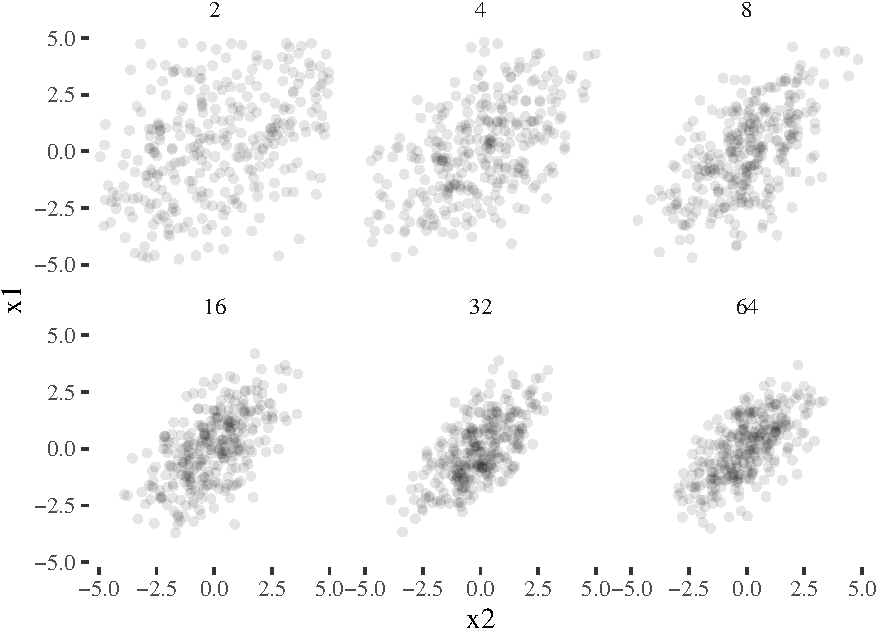
\includegraphics[width=500px]{figure-latex/scatter-1}
\caption[Distribution of Choices for Different Levels of
Optimality]{\label{scatter} Scatter plot of the choices $\mathbf{x_1}$ and
$\mathbf{x_2}$ for different levels (2, 4, 8, 16, 32, 64) of the optimality
parameter, $N$. The complementarity effect is fixed at $\beta_{12} = .5$ for all
samples. The decreasing marginal costs are set as $\delta_1 = \delta_2 = 1$. The
effect of the environmental variable only affects one of the choices
($\gamma_1 = .5, \gamma_2 = 0$). Lastly, the unobserved variation parameters are
set at $\sigma_{\epsilon_1} = \sigma_{\epsilon_2} = .5$ and $\sigma_{\nu} = 1.$}
\end{figure}

\subsection{Performance and Demand Function
Approach}\label{performance-and-demand-function-approach}

In the next section, we will compare the type I error rate and power of
the different statistical approaches when varying the optimality
parameter, \(N\). Because the accounting literature is concerned with
testing the hypothesis that there is (no) complementarity between two
management control practices, a focus on error rates and power is
appropriate. For brevity, we omit the results for the conditional
correlation specification as they are indistinguishable from the demand
function specification.

For each combination of parameters, we generate 1000 datasets of 300
observations, a typical dataset in the literature, and plot the t-static
for \(\beta^p_{12}\) and \(\beta^d_{12}\) in each dataset. The datasets
are created with the following fixed parameters,
\(\delta_1 = \delta_2 = 1\),
\(\sigma_{\epsilon_1} = \sigma_{\epsilon_2} = .5\) , and
\(\sigma_{\nu} = 1\). The parameters of interest, \(N\), \(\beta_{12}\),
\(\gamma_1\), and \(\gamma_2\) are varied across datasets. The
optimality parameter, \(N\), is manipulated as 2, 4, 8, 16, 32, and 64.
The complementarity is either present (\(\beta_{12} = 0.5\)) or the null
hypothesis is true (\(\beta_{12} = 0\)). The potentially confounding
environmental factor, \(\gamma_1\) and \(\gamma_2\), is either only
affecting one choice (\(\gamma_1 = .5, \gamma_2 = 0\)), or its effects
are positively correlated (\(\gamma_1 = \gamma_2 = .5\)), or negatively
correlated (\(\gamma_1 = .5\) and \(\gamma_2 = -.5\)).

Figure \ref{basic} shows the boxplot for the t-static for each type of
test and each combination of parameters. The dot represents the median
t-statistic of the 1000 datasets, the gap between the whiskers represent
the interquartile range, and the whiskers indicate the minimum and
maximum t-statistic. Each boxplot can be compared to the zero line and
the lines representing a 95\% confidence interval around a null effect.

\begin{figure}

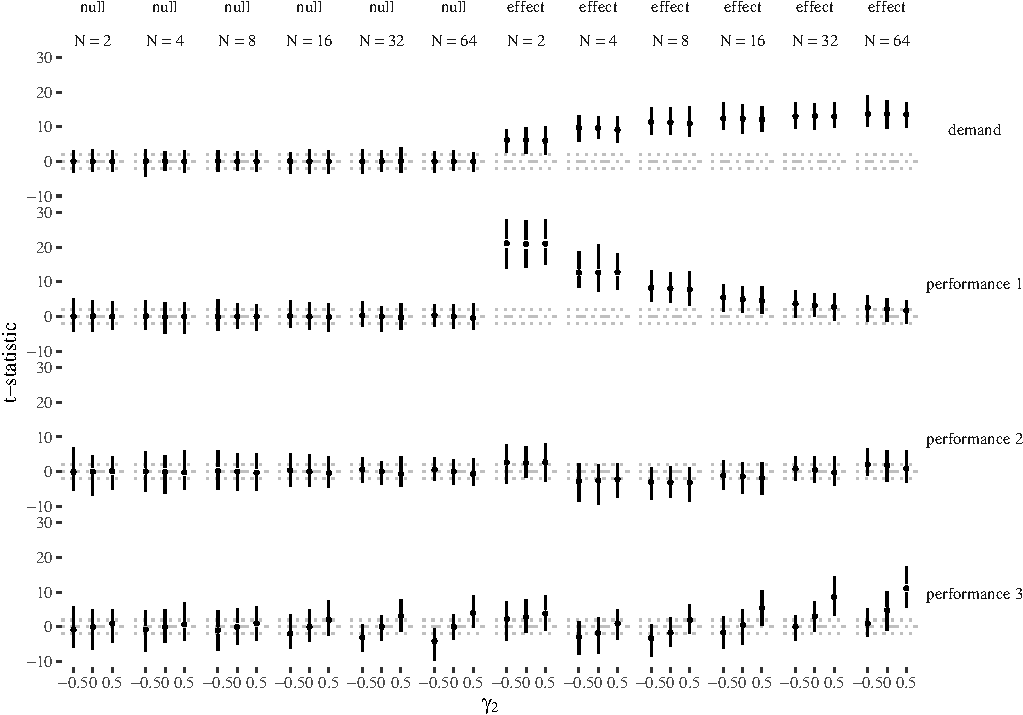
\includegraphics[width=500px]{figure-latex/unnamed-chunk-5-1}
\caption[Error Rate and Power of Demand and Performance Specification]
{\label{basic} t-static of the performance and demand approach to test
for complementarities when there is a complementarity effect ($\beta_{12} = .5$)
or a null ($\beta_{12} = 0$). The boxplots represent the median (the dot) the
interquartile range (the gap), and the minimum and maximum (the whiskers). $N$
is varied between 2, 4, 8, 16, 32, and 64. The effect of the environmental
variable, $\mathbf{z}$, on the second choice is either absent
($\gamma_1 = .5,  \gamma_2 = 0$), positive ($\gamma_1 = \gamma_2 = .5$),
or negative ($\gamma_1 = .5$ and $\gamma_2 = -.5$).}
\end{figure}

Figure \ref{basic} shows that the demand approach and the theoretically
derived \emph{performance 1} approach have on average a t-static close
to 0 in the absence of an interdependency. The figure also reveals the
basic trade-off between the demand approach and the performance
approach: with low levels of optimality the performance function is more
likely to detect a true complementarity effect while the demand function
is more likely to detect a true complementarity effect with high levels
of optimality \citep{Grabner2013, Aral2012}. Interestingly, even at
relatively low levels of optimality, \(N = 4\), the demand approach has
similar power to the \emph{performance 1} approach. That is, if firms
avoid the worst possible combinations (see Figure \ref{scatter}), the
demand approach has the power to detect a true effect.

The \emph{performance 2} and \emph{3} specification fare worse compared
to the theoretically appropriate specifications. Both drop the quadratic
effects that control for decreasing marginal costs. In addition,
\emph{performance 3} does not control for the interactions
\(\mathbf{x_1z}\) and \(\mathbf{x_2z}\). The latter omission effects the
estimate for the complementarity even with a null effect. Figure
\ref{basic} shows that when \(\gamma_2 \neq 0\), the median t-statistic
diverges from 0 and the divergence increases with the level of
optimality. The intuition behind this result is that with higher levels
of optimality and when \(\gamma_1 \gamma_2 \neq 0\), the environmental
factor is correlated with the management controls and hence the
interactions, \(\mathbf{x_1z}\) and \(\mathbf{x_2z}\), are correlated
with the interaction \(\mathbf{x_1 x_2}\). Omitting the interactions
between the environmental factors and the management accounting choices,
biases the estimates of the interdependency,
\(\beta_{12}^{p3} \mathbf{x_1 x_2}\).

The most dramatic effects of the omitted correlated variables can be
observed when a true interdependency exists. When the optimality
parameter exceeds 4, the \emph{performance 2} and \emph{performance 3}
specification are unlikely to detect the true effect,
\(\beta_{12} = .5\), and are under some circumstances likely to report a
substitution effect. The latter results shows that the performance
approaches currently used in the management accounting literature are
inappropriate to test for interdependencies with most parameter
combinations in this simulation.

\begin{table}[ht]
\centering
\begingroup\footnotesize
\begin{tabular}{lrlrrrrrr}
  \hline
method & $\gamma_2$ & type & 2 & 4 & 8 & 16 & 32 & 64 \\
  \hline
demand & -0.50 & type I & 0.03 & 0.04 & 0.04 & 0.04 & 0.04 & 0.04 \\
  demand & 0.00 & type I & 0.03 & 0.04 & 0.03 & 0.04 & 0.05 & 0.04 \\
  demand & 0.50 & type I & 0.05 & 0.03 & 0.04 & 0.04 & 0.04 & 0.03 \\
  performance~1 & -0.50 & type I & 0.14 & 0.13 & 0.13 & 0.12 & 0.10 & 0.08 \\
  performance~1 & 0.00 & type I & 0.14 & 0.12 & 0.11 & 0.12 & 0.08 & 0.08 \\
  performance~1 & 0.50 & type I & 0.14 & 0.13 & 0.10 & 0.11 & 0.10 & 0.10 \\
  performance~2 & -0.50 & type I & 0.23 & 0.27 & 0.26 & 0.21 & 0.14 & 0.11 \\
  performance~2 & 0.00 & type I & 0.22 & 0.25 & 0.23 & 0.19 & 0.12 & 0.09 \\
  performance~2 & 0.50 & type I & 0.22 & 0.25 & 0.23 & 0.18 & 0.14 & 0.13 \\
  performance~3 & -0.50 & type I & 0.28 & 0.30 & 0.32 & 0.52 & 0.80 & 0.95 \\
  performance~3 & 0.00 & type I & 0.21 & 0.23 & 0.22 & 0.17 & 0.11 & 0.09 \\
  performance~3 & 0.50 & type I & 0.28 & 0.27 & 0.31 & 0.51 & 0.79 & 0.96 \\
  demand & -0.50 & power & 1.00 & 1.00 & 1.00 & 1.00 & 1.00 & 1.00 \\
  demand & 0.00 & power & 1.00 & 1.00 & 1.00 & 1.00 & 1.00 & 1.00 \\
  demand & 0.50 & power & 1.00 & 1.00 & 1.00 & 1.00 & 1.00 & 1.00 \\
  performance~1 & -0.50 & power & 1.00 & 1.00 & 1.00 & 1.00 & 0.94 & 0.76 \\
  performance~1 & 0.00 & power & 1.00 & 1.00 & 1.00 & 1.00 & 0.86 & 0.58 \\
  performance~1 & 0.50 & power & 1.00 & 1.00 & 1.00 & 0.98 & 0.74 & 0.40 \\
  performance~2 & -0.50 & power & 0.66 & 0.00 & 0.00 & 0.01 & 0.18 & 0.56 \\
  performance~2 & 0.00 & power & 0.64 & 0.00 & 0.00 & 0.00 & 0.10 & 0.45 \\
  performance~2 & 0.50 & power & 0.70 & 0.00 & 0.00 & 0.00 & 0.04 & 0.23 \\
  performance~3 & -0.50 & power & 0.57 & 0.00 & 0.00 & 0.00 & 0.06 & 0.20 \\
  performance~3 & 0.00 & power & 0.70 & 0.01 & 0.01 & 0.15 & 0.78 & 0.97 \\
  performance~3 & 0.50 & power & 0.89 & 0.22 & 0.50 & 0.99 & 1.00 & 1.00 \\
   \hline
\end{tabular}
\endgroup
\caption[Error Rate and Power of the Demand and Performance Specification]{Type I error rates and power for the demand and
performance specification at different levels optimality: 2, 4, 8,
16, 32, 64. The parameters are the same as in Figure \ref{basic}.}
\label{basic-error}
\end{table}

To investigate the performance of the demand and performance
specifications in more detail, we report the type I error rate and power
based on the simulations in Table \ref{basic-error}. The type I error is
the percentage of datasets with no complementarity where the t-statistic
of \(\beta^d_{12}\) is higher than \(1.97\) or lower than \(-1.97\). The
power is the percentage of datasets with a real effect where the
t-statistic exceeds \(1.97\). An important caveat is that the power of a
study will also be influenced by measurement error, random variation and
the number of observations in the study. In the simulations, we assumed
no measurement error, fixed the parameters that control random
variation, \(\sigma_{\epsilon_1}\), \(\sigma_{\epsilon_2}\), and
\(\sigma_{\nu}\), and the number of observations per dataset. As a
result, the numbers in Table \ref{basic-error} should be interpreted
with caution.

Under the parameters in the simulation study, the \emph{demand} approach
has type I error rates slightly below the nominal value of \(0.05\). The
theoretically appropriate \emph{performance 1} specification tends to
have more elevated error rates, two to three times higher than for the
\emph{demand} specification. The most worrying results are for the
\emph{performance 2} and \emph{3} specification. Dropping the quadratic
effects increases the error rates in the \emph{performance 2}
specification to around \(.20\), four times the nominal error rate. The
most common specification in the literature, \emph{performance 3}, has
even higher type I error rates that increase with higher levels of
optimality and when the effectiveness of both management controls varies
with the environmental factor. In conclusion, with the parameters in the
simulation study only the \emph{demand} specification rejects the null
hypothesis at the predetermined rate. While the theoretically derived
\emph{performance 1} specification has slightly elevated error rates,
the two other performance approaches are vulnerable to false positives.

The results for the power of the different specifications shows that
with the parameters in the simulation, the trade-off between the demand
specification and the performance specification is a second order
problem when using the theoretically derived specification. Both the
\emph{demand} and the \emph{performance 1} specification are able to
detect a true interdependency with almost certainty for low to medium
levels of optimality. However, the \emph{demand} specification is more
likely to detect a true effect at higher levels of optimality. The
reduced specifications \emph{performance 2} and \emph{3} are not able to
detect the true interdependency for most of the parameter space under
investigation. They are more likely to report a significant negative
interdependency than the true positive interdependency.

One way to interpret this result is to think about how a reader should
react when observing a study with a significant positive interaction
\(\mathbf{x_1 x_2}\). To demonstrate the problems with the
\emph{performance 2} and \emph{3} specification, we provide one dramatic
example for \(N = 4\) and \(\gamma_2 = -.05\). If we assume that a
priori, we are indifferent between a null effect and a true
interdependency of \(\beta_{12} = 0.5\), and we observe one study that
reports a significant positive interaction \(\mathbf{x_{1} x_{2}}\), the
study is more likely to be from a sample where the null holds than from
a sample where there is a true interdependency!

\subsection{Parameter Variations}\label{parameter-variations}

In this section, we explore the robustness of the above conclusions to
variations in the structural parameters. Given the large number of
possible variations, we restrict ourselves to theoretically driven
comparisons.

\subsubsection{Unobserved Performance
Effects}\label{unobserved-performance-effects}

We first investigate whether increases in the variance of performance,
\(\sigma_{\nu}\), change the conclusions. The first effect of increasing
the variance is that it decreases the importance of the management
controls for performance which decreases the power of the performance
specification. The second effect follows from the first. When the
management controls are less important, the optimality selection effects
are less pronounced which in turn decreases the power of the demand
specification and the omitted correlated variable bias in the
\emph{performance 2} and \emph{performance 3} specification.

To investigate the role of \(\sigma_{\nu}\), we vary the parameter
between 1, 2, and 4 while keeping most of the other parameters the same
as in Figure \ref{basic-error}. For clarity of exposition, we limit the
number of optimality variations (\(N = 2, 8, 32\)) and the number of
variations of the moderating effect of \(\mathbf{x_2 z}\)
(\(\gamma_2 = -.5, .5\)).

The results in Figure \ref{noise} and Table \ref{noise-error} are not
qualitatively different from the previous results. The \emph{demand} and
\emph{performance 1} specification appear largely unbiased and have
false positive rates below or close to the nominal rates. The
\emph{performance 2} and \emph{performance 3} specification exhibit the
same problem as before, elevated false positive rates as the result of
omitted correlated variables. The increase in unobserved performance
variation does lessen the impact of the bias.

More importantly, in the presence of an interdependency, the increase in
performance variance hardly effects the performance of the \emph{demand}
specification. For every simulated dataset with a real interdependency
the \emph{demand} specification, correctly identifies this
interdependency although the t-statistics decrease with higher
performance variance. The drop-off in the t-statistic is steeper for the
\emph{performance 1} specification to the extent that power drops to
around \(50\%\) when \(N = 32\) and \(\sigma_{\nu} = 4\). In summary,
these results indicate that the major impact of increasing the
performance variance is to decrease the power of the performance
specifications and only to a lesser extent decrease the effect of the
optimality parameter.

\begin{figure}

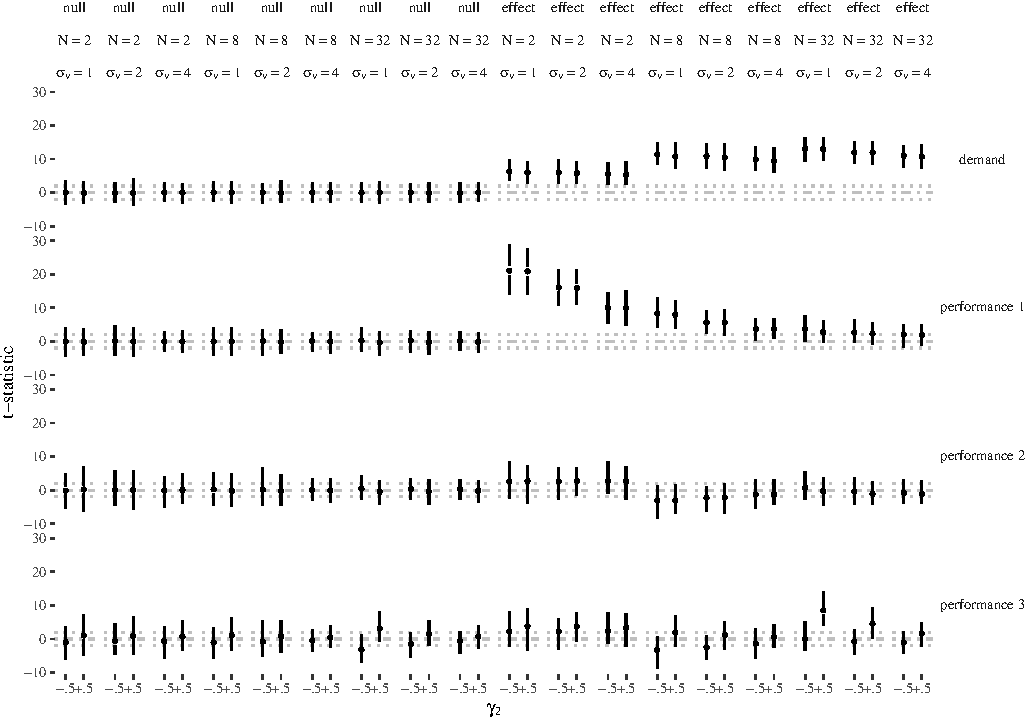
\includegraphics[width=500px]{figure-latex/unnamed-chunk-7-1}
\caption[Error Rate and Power with Increasing Levels of Variability in Performance]
{\label{noise} t-static of the performance and demand approach to test
for complementarities when there is a complementarity effect ($\beta_{12} = .5$)
or a null ($\beta_{12} = 0$). The boxplots represent the median (the dot) the
interquartile range (the gap), and the minimum and maximum (the whiskers). $N$
is varied between 2, 8, 32. The effect of the environmental
variable, $\mathbf{z}$, on the second choice is either positive
($\gamma_1 = \gamma_2 = .5$), or
negative ($\gamma_1 = .5$ and $\gamma_2 = -.5$).}
\end{figure}

\begin{table}[ht]
\centering
\begingroup\footnotesize
\begin{tabular}{lrrlrrr}
  \hline
method & $\gamma_2$ & $\sigma_{\nu}$ & type & 2 & 8 & 32 \\
  \hline
demand & -0.50 & 4.00 & type I & 0.03 & 0.04 & 0.04 \\
  demand & 0.50 & 4.00 & type I & 0.04 & 0.03 & 0.05 \\
  performance~1 & -0.50 & 4.00 & type I & 0.06 & 0.05 & 0.04 \\
  performance~1 & 0.50 & 4.00 & type I & 0.06 & 0.04 & 0.05 \\
  performance~2 & -0.50 & 4.00 & type I & 0.14 & 0.08 & 0.06 \\
  performance~2 & 0.50 & 4.00 & type I & 0.16 & 0.07 & 0.06 \\
  performance~3 & -0.50 & 4.00 & type I & 0.19 & 0.10 & 0.12 \\
  performance~3 & 0.50 & 4.00 & type I & 0.18 & 0.10 & 0.10 \\
  demand & -0.50 & 4.00 & power & 1.00 & 1.00 & 1.00 \\
  demand & 0.50 & 4.00 & power & 1.00 & 1.00 & 1.00 \\
  performance~1 & -0.50 & 4.00 & power & 1.00 & 0.95 & 0.56 \\
  performance~1 & 0.50 & 4.00 & power & 1.00 & 0.94 & 0.47 \\
  performance~2 & -0.50 & 4.00 & power & 0.70 & 0.00 & 0.00 \\
  performance~2 & 0.50 & 4.00 & power & 0.69 & 0.00 & 0.00 \\
  performance~3 & -0.50 & 4.00 & power & 0.61 & 0.00 & 0.00 \\
  performance~3 & 0.50 & 4.00 & power & 0.84 & 0.11 & 0.37 \\
   \hline
\end{tabular}
\endgroup
\caption[Error Rate and Power with Increasing Levels of Variability in Performance]{Type I error rates and power for the demand and
performance function approaches at different levels optimality: 2, 8, 32 The
parameters are the same as in Figure \ref{noise}. For brevity, we only report the
results for $\sigma_{\nu} = 4$}
\label{noise-error}
\end{table}

\subsubsection{Marginal Cost Effects}\label{marginal-cost-effects}

In this section, we vary the size of the increase in marginal costs,
\(\delta_1\) = \(\delta_2\). We keep the parameters the same for both
management control practices but they become smaller in size. In the
next section, we investigate the effect of asymmetrically increasing
marginal costs.

There are two consequences of lowering the increase in marginal costs.
First, the bias from omitting the quadratic terms should be smaller.
Second, decreasing \(\delta_1 = \delta_2\) also increases the effect of
optimality by increasing the conditional correlation between the
management control practices. With \(r=0\), we know from equation
\(\eqref{eq:conditional}\) that the conditional correlation,
\(\rho^*_c\), depends on two parameters, \(\beta\) and \(\Delta\). While
\(\Delta\) is only affected by the ratio \(\frac{\delta_1}{\delta_2}\),
\(\beta = \frac{\beta_{12}}{\sqrt{\delta_1 \delta_2}}\) is determined by
the size of the complementarity and the product of the decreasing
marginal costs. When \(\delta_1 \delta_2\) increases, so thus \(\beta\)
and the conditional correlation.

In Figure \ref{basic} and \ref{noise}, we used
\(\delta_1 = \delta_2 = 1\). In this section, we investigate two other
values 0.5 and 0. \(\delta_1 = \delta = .5\) is the largest value for
which the parameters violates the second-order optimality condition
\(\beta_{12} < \sqrt{\delta_1 \delta_2}\). The extreme case is when
\(\delta_1 = \delta_2 = 0\) which may impede the performance of the
\emph{demand} specification even further.

\begin{figure}

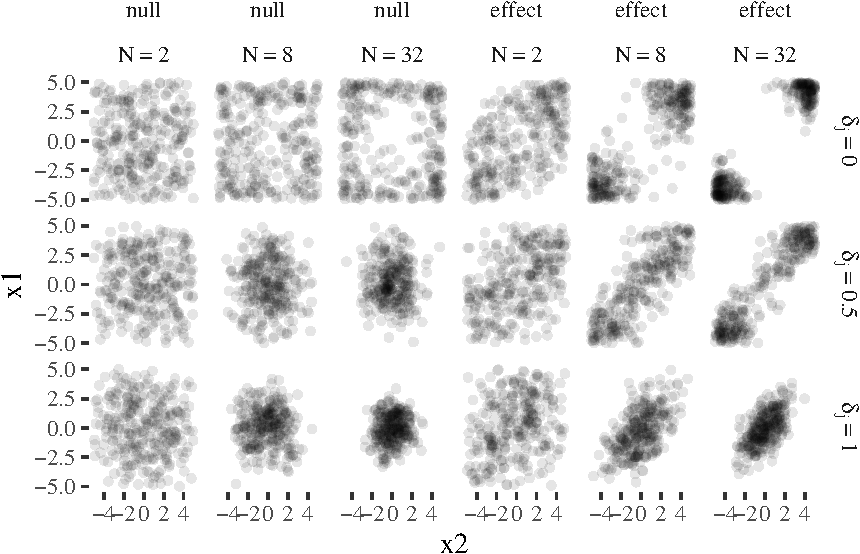
\includegraphics[width=500px]{figure-latex/scatterplot-delta-1}
\caption[Error Rate and Power with Different Levels of Marginal
Costs]{\label{scatter-delta} Scatter plot of the choices $\mathbf{x_1}$ and
$\mathbf{x_2}$ for different levels (2, 8, 32) of the optimality parameter, $N$
with a null interdependency ($\beta_{12} = 0$) or a true effect ($\beta_{12} =
0$). The increasing marginal costs are set as $\delta_1 = \delta_2 = 0, 0.5$,
and $1$. The effect of the environmental variable only affects one of the
choices ($\gamma_1 = .5, \gamma_2 = 0$). Lastly, the unobserved variation
parameters are set at $\sigma_{\epsilon_1} = \sigma_{\epsilon_2} = .5$ and
$\sigma_{\nu} = 1.$ }
\end{figure}

To visualise those effects on a simulated sample, we first generate a
dataset for three levels of optimality and three values of
\(\delta_1 = \delta_2\) and plot the values for \(\mathbf{x_1}\) and
\(\mathbf{x_2}\) in a scatterplot. Figure \ref{scatter-delta} shows when
marginal costs are constant, the practices, \(\mathbf{x_1}\) and
\(\mathbf{x_2}\), are pushed towards the boundary values especially when
there is a complementarity and with higher levels of optimality. At the
intermediate level, \(\delta_1 = \delta_2 = 0.5\), the choices cluster
around the origin with the null effect, while they are pushed toward the
boundaries with a true interdependency. The large variations between the
scatterplots show how visual inspection can help researchers to check
whether the underlying assumption of their statistical test are met. A
pattern to look for is whether the values for the choices are at the
boundaries of the measurement scale (for small \(\delta_j\)) or not (for
larger \(\delta_j\)).

In Figure \ref{delta} and Table \ref{delta-error}, we report the
performance of the different specifications to detect an
interdependency. Especially at lower levels of optimality, the
\emph{demand} approach suffers from elevated false positives when the
marginal costs of the choices are constant. Under these conditions, the
\emph{performance 1} specification is more appropriate to protect the
null hypothesis. Nevertheless, the power of the \emph{demand approach}
is generally better for all but the lowest level of optimality.
Furthermore, the \emph{performance 1} approach suffers from steeper
decreases in power as the result of increases in optimality.

\begin{figure}

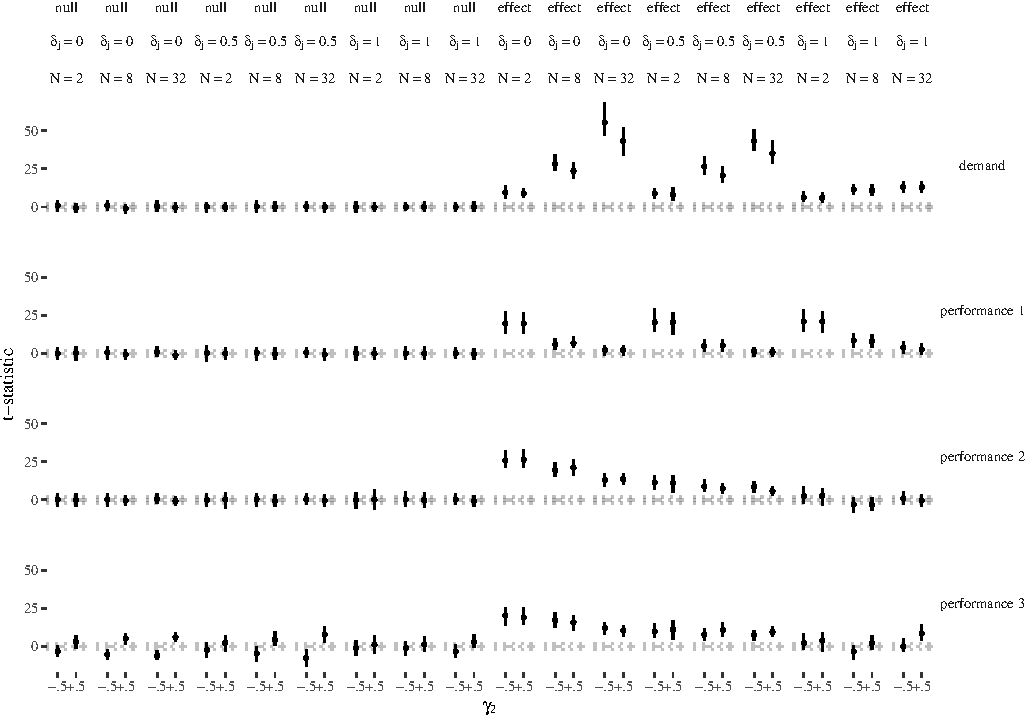
\includegraphics[width=500px]{figure-latex/unnamed-chunk-9-1}
\caption[The Error Rate and Power with Different Levels of Marginal Costs]
{\label{delta} t-static of the performance and demand approach to test
for complementarities when there is a complementarity effect ($\beta_{12} = .5$)
or a null ($\beta_{12} = 0$). The boxplots represent the median (the dot) the
interquartile range (the gap), and the minimum and maximum (the whiskers). $N$
is varied between 2, 8, 32. The effect of the environmental
variable, $\mathbf{z}$, on the second choice is either positive
($\gamma_1 = \gamma_2 = .5$), or negative ($\gamma_1 = .5$ and $\gamma_2 = -.5$).
The increasing marginal costs varied between $\delta_1 = \delta_2 = 0, .5, 1$}
\end{figure}

\begin{table}[ht]
\centering
\begingroup\footnotesize
\begin{tabular}{lrrlrrr}
  \hline
method & $\gamma_2$ & $\delta_{j}$ & type & 2 & 8 & 32 \\
  \hline
demand & -0.50 & 0.00 & type I & 0.14 & 0.17 & 0.08 \\
  demand & 0.50 & 0.00 & type I & 0.14 & 0.15 & 0.07 \\
  demand & -0.50 & 0.50 & type I & 0.05 & 0.04 & 0.05 \\
  demand & 0.50 & 0.50 & type I & 0.04 & 0.03 & 0.05 \\
  demand & -0.50 & 1.00 & type I & 0.05 & 0.03 & 0.04 \\
  demand & 0.50 & 1.00 & type I & 0.05 & 0.04 & 0.04 \\
  performance~1 & -0.50 & 0.00 & type I & 0.11 & 0.11 & 0.18 \\
  performance~1 & 0.50 & 0.00 & type I & 0.11 & 0.11 & 0.19 \\
  performance~1 & -0.50 & 0.50 & type I & 0.12 & 0.12 & 0.14 \\
  performance~1 & 0.50 & 0.50 & type I & 0.14 & 0.12 & 0.14 \\
  performance~1 & -0.50 & 1.00 & type I & 0.12 & 0.12 & 0.10 \\
  performance~1 & 0.50 & 1.00 & type I & 0.15 & 0.13 & 0.11 \\
   \hline
\end{tabular}
\endgroup
\caption[Error Rate and Power with Different Levels of Marginal Costs]{ Type I error rates for the demand and performance 1
approaches at different levels optimality: 2, 8, 32 The parameters are the same
as in Figure \ref{delta}.}
\label{delta-error}
\end{table}

\subsubsection{Asymmetrically increasing marginal
costs}\label{asymmetrically-increasing-marginal-costs}

The next variation we investigate are changes in the ratio
\(\frac{\delta_1}{\delta_2}\) while keeping \(\delta_1 \delta_2 = 1\).
This means that costs are increasing faster for one practice than for
the other. The ratio affects the conditional correlation only through
the parameter, \(\Delta\) (see equation \eqref{eq:conditional}). When
\(\delta_1\) and \(\delta_2\) are more different, \(\Delta\) increases,
and \(|\rho^*_c|\) gets closer to \(1\). In addition, as can be seen
from equation \eqref{eq:demand2}, the standard deviation of
\(\mathbf{x_1}\) (\(\mathbf{x_2}\)) increases when \(\delta_2\)
(\(\delta_1\)) increases and vice versa. Both effects, can be seen in
Figure \ref{scatter-delta} for the following values of
\(\delta_1 = \delta_2^{-1}\): \(1/3\), \(1\), and \(3\) \footnote{Equation
  \eqref{eq:coefficient} shows that the standard deviations of
  \(\mathbf{x_1}\) and \(\mathbf{x_2}\) also effect the regression
  estimate \(\beta_{12}^d\). As a result, the conditional correlation
  and the regression demand specification could be expected to yield
  different results. The simulation results show that the differences in
  the t-statistic are merely due to numerical differences. As before,
  for brevity we only report the results for the \emph{demand}
  regression specification.}.

\begin{figure}

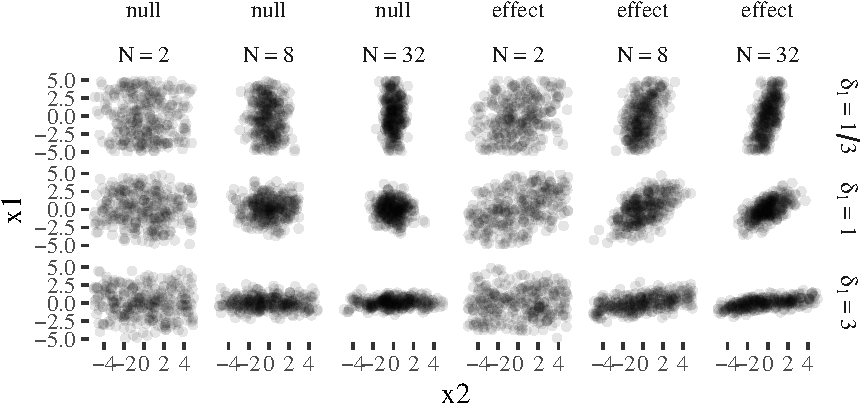
\includegraphics[width=500px]{figure-latex/scatterplot-delta2-1}
\caption[Distribution of Choices with Asymmetric Marginal Costs]
{\label{scatter-delta2} Scatter plot of the choices $\mathbf{x_1}$ and
$\mathbf{x_2}$ for different levels (2, 8, 32) of the optimality parameter, $N$
with a null interdependency ($\beta_{12} = 0$) or a true effect
($\beta_{12} = 0$). The increasing marginal costs are set as
$\delta_1 = \delta_2^{-1} = 1/3$,$1$, and $3$. The effect of the environmental
variable only affects one of the choices ($\gamma_1 = .5, \gamma_2 = 0$).
Lastly, the unobserved variation parameters are set at
$\sigma_{\epsilon_1} = \sigma_{\epsilon_2} = .5$ and $\sigma_{\nu} = 1.$ }
\end{figure}

The simulation results in Figure \ref{scatter-delta2} show that the
effects of asymmetrically increasing marginal costs is relatively small.
The general trends for both error rates and power remain the same. The
\emph{demand} approach has superior error rates and, except for low
levels of optimality, most power to detect a real effect. The
\emph{performance 2} and \emph{performance 3} specifications perform
badly. Nevertheless, asymmetrically increasing marginal costs decrease
the power of the \emph{demand} specification and increase the power of
the \emph{performance 1} specification, especially with lower levels of
optimality.

\begin{figure}

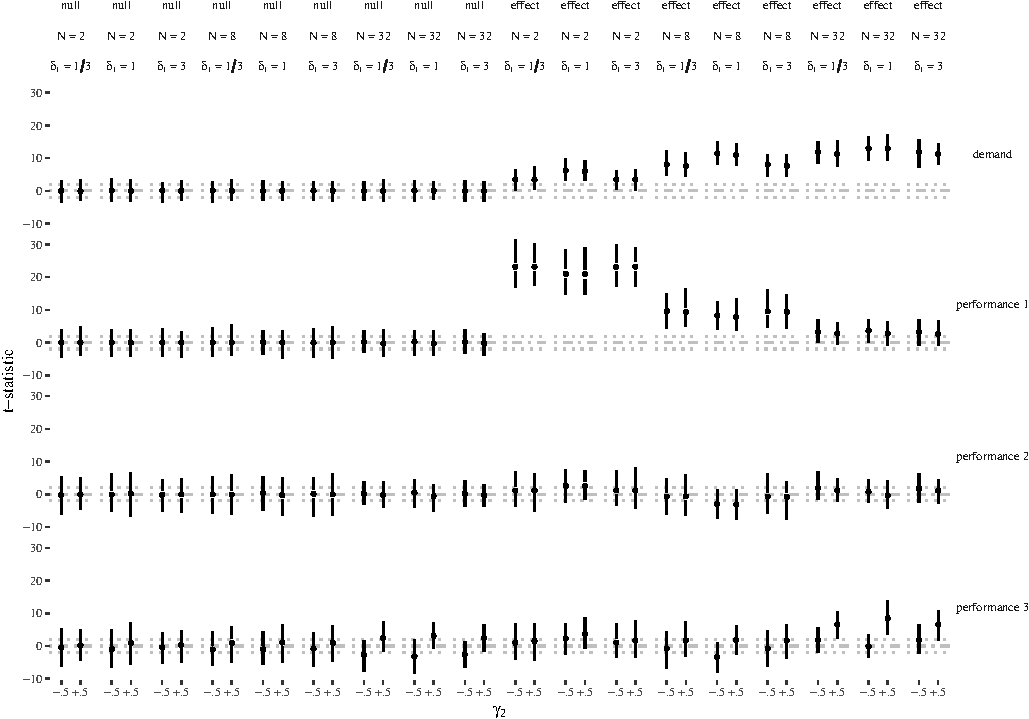
\includegraphics[width=500px]{figure-latex/unnamed-chunk-10-1}
\caption[Error Rate and Power with Asymmetric with Marginal Costs]
{\label{delta2} t-static of the performance and demand specification to test
for complementarities when there is a complementarity effect ($\beta_{12} = .5$)
or a null ($\beta_{12} = 0$). The boxplots represent the median (the dot) the
interquartile range (the gap), and the minimum and maximum (the whiskers). $N$
is varied between 2, 8, 32. The effect of the environmental
variable, $\mathbf{z}$, on the second choice is either positive
($\gamma_1 = \gamma_2 = .5$), or
negative ($\gamma_1 = .5$ and $\gamma_2 = -.5$). The increasing marginal costs
are varied at $\delta_1 = \delta_2^{-1} = 1/3, 1$ and $3$}
\end{figure}

\subsection{Spurious correlation}\label{spurious-correlation}

Finally, we investigate to what extent a spurious correlation induced by
an omitted correlated environmental factor affects our conclusions. From
equation \eqref{eq:conditional}, we know that with optimal choices and a
spurious correlation, the \emph{demand} specification leads to type I
errors. In this section, we assume a well designed study that controls
for most of the environmental factors affecting the performance of both
choices. Based on prior literature, we determine reasonable values for
the effect of an unobserved factor on the performance effect of both
choices. Under the assumption of optimal choices, these effects will
show up as correlations between the choices and the environmental
factors (see also Equation \eqref{eq:demand2}). To calibrate the
parameters in the simulation, we use 5 recent studies that investigate
interdependencies between management control choices and report
correlations between the choices and environmental factors
\citep{Dekker2016, Grabner2016, Bedford2015, Heinicke2016, Abernethy2015a}\footnote{\citet{Grabner2016},
  \citet{Bedford2015}, \citet{Heinicke2016}, \citet{Abernethy2015a}
  report similar sized correlations between choices and between choices
  and environmental factors. In a study on interfirm collaborations
  \citet{Dekker2016} reports higher correlation both between choices and
  between choices and environmental factors.}. Those studies report
307\footnote{\citet{Bedford2015} has by far the biggest contribution
  with 264 correlations.} correlations between practices and
environmental factors with the average of the median correlation per
study equal to .18 and the average of the average correlation equal to
.21. We assume that a well designed study has not excluded any
environmental factor that correlates stronger than .25 with both
choices.

To test the vulnerability of the \emph{demand} specification and the
\emph{performance 1} specification to spurious correlations in a well
designed study, we run the following simulation. We introduce a new
unobserved environmental factor \(\mathbf{w}\) that impacts the
performance effect of \(\mathbf{x_1}\) with \(\theta_1\) and the
performance effect of \(\mathbf{x_2}\) with \(\theta_2\) (See the
Appendix for the full specification). We set \(\theta_1 = .25\) and vary
\(\theta_2 = .-25, -0.125, -0.0625\) to introduce a negative spurious
correlation which could lead to higher type I errors and less power to
detect a complementarity effect. To better illustrate the latter, we
introduce a medium sized interdependency of \(\beta_{12} = .25\) next to
the null effect \(\beta_{12} = 0\) and the large interdependency
\(\beta_{12} = .5\).

The results of the simulation are reported in Figure \ref{spurious} and
Table \ref{spurious-error}. The results are consistent with our previous
findings. The \emph{demand} specification has superior type I error
rates than the \emph{performance 1} specification and at all but the
lowest levels of optimality, the \emph{demand} specification has at
least the same power to detect a true interdependency as the
\emph{performance 1} specification. One important finding is that the
\emph{demand} specification becomes more vulnerable to type I error
rates when there is a null effect under higher levels of optimality.
This effect is most pronounced with the largest spurious correlation
(\(\theta_1 = .25\), \(\theta_2 = -.25\)) where we find that in 14\% of
the simulations with a null effect the \emph{demand} specification
reports a significant effect. The finding reinforces that the
\emph{demand} specification will only have appropriate type I error
rates as part of a well designed study that controls for environmental
factors that affect both choices especially when firms adopt the optimal
management controls.

\begin{figure}

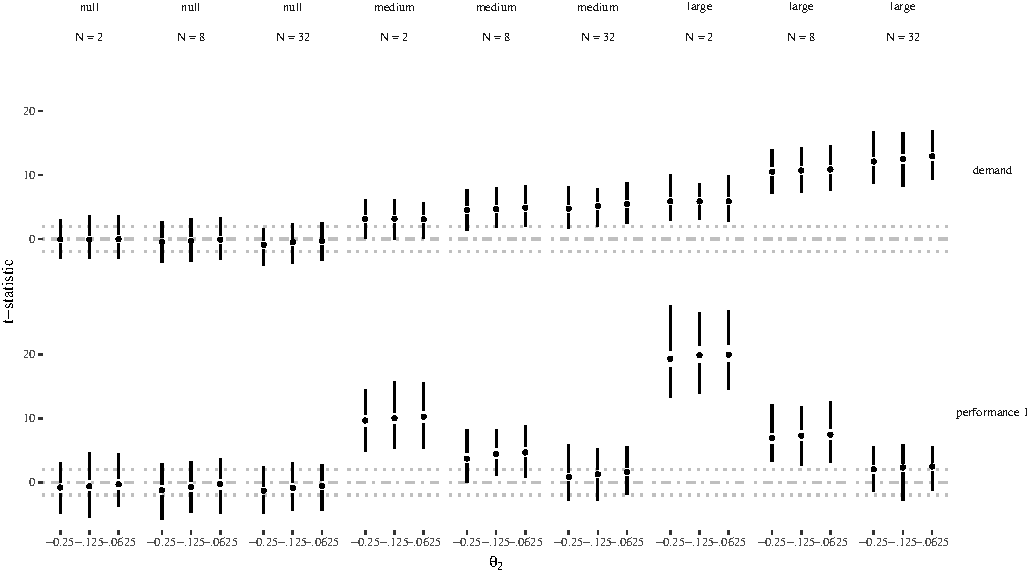
\includegraphics[width=500px]{figure-latex/spurious-plot-1}
\caption[Error Rate and Power with Unobserved Environmental Variables]
{\label{spurious} t-static of the performance and demand specification to test
for complementarities when there is a large complementarity effect
($\beta_{12} = .5$), a medium complementarity effect ($\beta_{12} = .25$),
or a null ($\beta_{12} = 0$). The boxplots represent the median (the dot) the
interquartile range (the gap), and the minimum and maximum (the whiskers). $N$
is varied between 2, 8, 32. The effect of the unobserved environmental variable,
$\mathbf{w}$, on the choices varies from mildly correlated ($\theta_1 = .25$,
$\theta_2 = -.25$), ($\theta_1 = .25$ and $\theta_2 = -.125$),
to weakly correlated ( $\theta_1 =.25$, $\theta_2 = -.0.0625$). The increasing
marginal costs are set at $\delta_1 = \delta_2 = 1$}.
\end{figure}

\begin{table}[ht]
\centering
\begingroup\footnotesize
\begin{tabular}{llrlrrr}
  \hline
method & effect & $\theta_2$ & type & 2 & 8 & 32 \\
  \hline
demand & null & -0.2500 & type I & 0.05 & 0.07 & 0.14 \\
  demand & null & -0.1250 & type I & 0.04 & 0.05 & 0.06 \\
  demand & null & -0.0625 & type I & 0.04 & 0.04 & 0.05 \\
  performance~1 & null & -0.2500 & type I & 0.22 & 0.28 & 0.29 \\
  performance~1 & null & -0.1250 & type I & 0.18 & 0.20 & 0.19 \\
  performance~1 & null & -0.0625 & type I & 0.15 & 0.15 & 0.12 \\
  demand & medium & -0.2500 & power & 0.89 & 1.00 & 1.00 \\
  demand & medium & -0.1250 & power & 0.88 & 1.00 & 1.00 \\
  demand & medium & -0.0625 & power & 0.89 & 1.00 & 1.00 \\
  demand & large & -0.2500 & power & 1.00 & 1.00 & 1.00 \\
  demand & large & -0.1250 & power & 1.00 & 1.00 & 1.00 \\
  demand & large & -0.0625 & power & 1.00 & 1.00 & 1.00 \\
  performance~1 & medium & -0.2500 & power & 1.00 & 0.92 & 0.15 \\
  performance~1 & medium & -0.1250 & power & 1.00 & 0.98 & 0.27 \\
  performance~1 & medium & -0.0625 & power & 1.00 & 0.97 & 0.37 \\
  performance~1 & large & -0.2500 & power & 1.00 & 1.00 & 0.52 \\
  performance~1 & large & -0.1250 & power & 1.00 & 1.00 & 0.63 \\
  performance~1 & large & -0.0625 & power & 1.00 & 1.00 & 0.66 \\
   \hline
\end{tabular}
\endgroup
\caption[Error Rate and Power with Unobserved Environmental Variables]{Type I error rates for the demand and performance 1
approaches at different levels optimality: 2, 8, 32. Theparameters are the same
as in Figure \ref{spurious}.}
\label{spurious-error}
\end{table}

\section{Summary and discussion}\label{summary-and-discussion}

This study builds on earlier studies on complementarity theory
\citep{Milgrom1995, Grabner2013}, to provide guidance on how to test for
the presence of interdependencies in management control systems. The
results of the simulation study show that in most common scenarios the
assumptions of optimality should not be the main driver in deciding
between the demand or the performance specification. In fact, unless the
researchers can make the case that a large number of firms will have a
highly dysfunctional management control design, the demand specification
should be the preferred statistical method. A straight-forward check on
the optimality assumption is to investigate the correlation between the
practices and the environmental variables. Non-trivial levels of
optimality will induce correlations between management accounting
practices and environmental factors when there are contingency effects.
Nevertheless, it is important to note that the absence of any
correlations does not imply the absence of high levels of optimality as
multiple contingency effects can cancel each other out\footnote{An other
  clarification about the superiority of the demand specification is
  that it does not imply that the demand function approach provides
  evidence for high levels of optimality. A statistically significant
  interdependency effect in the demand specification only implies that
  firms on average avoid the worst possible management control systems,
  not that they have on average the optimal control system.}.

When performance data is available, the performance specification can be
estimated as an additional test in combination with the demand
specification. The performance function approach can be expected to
yield acceptable estimates when there is enough performance variation
between firms. However, the results of this study show the importance of
adequately controlling for environmental factors and potential
non-linear performance effects. As far as we know, the current
accounting literature does not fully address these correlated omitted
variable problems which lead to substantial increases in type I error
rates and a loss of power.

The most important weakness of the demand function approach is that it
assumes that the performance benefits of management control practices
are decreasing with more extensive use. If this second-order condition
does not hold, the demand approach will have elevated levels of false
positives. We suggest that researchers verify the distribution of the
management practices to check whether the second-order condition holds.
If one of the management practices has more observations at the extremes
of the measurement scale than at the center, the second-order condition
might be violated and the results of both the demand and performance
specification should be interpreted with care.

This study has several limitations. Both approaches under investigations
have their shortcomings. Our preferred approach, the demand
specification, does not allow to directly estimate the performance
effect of the interdependency. More sophisticated models are needed to
reliably estimate this performance effect. The economics literature has
proposed and used a multiple equation model that combines both demand
and performance functions
\citep{Athey1998, Gentzkow2007, Kretschmer2012, Miravete2006}. Further
research can investigate the appropriateness of these statistical models
for the management control setting. An additional advantage of the
models is that they can incorporate the effect of unobserved contingency
factors and unobserved interdependent practices. A more detailed
discussion of these issues goes beyond the scope of this study.

Another limitation of the current study is that the level of optimality
is implemented with a naive algorithm that lacks external validity.
Better theoretical models of how firms choose management accounting
practices can improve upon our understanding of the distribution of
management accounting practices and their interdependencies. The
approach of Hemmer and Labro \citeyearpar{Hemmer2015} is one potential
avenue to further explore. They model the firm's choices as decisions
under incomplete information with Bayesian updating when more
information becomes available. In these models, firms can end up with
ex-post sub-optimal management control systems because they lack the
appropriate information to choose the optimal system. The parameter
governing the lack of information can replace our optimality parameter,
\(N\). Further innovations in these models can allow researchers to
directly estimate the extent to which firms lack information and choose
sub-optimal management control practices.

\pagebreak

\appendix
\renewcommand{\theequation}{A.\arabic{equation}}
\setcounter{equation}{0}

\section{Appendix}\label{appendix}

\subsection{Quotes}\label{correlation-interaction}

\begin{quote}
Which {[}specification{]} to use is both a theoretical (assumption of agents as perfectly or boundedly rational) and an empirical (market imperfections, exogenous shocks, experimentation, etc) issue because the likelihood of finding evidence of the former depends on the latter and vice versa (Grabner and Moers, 2013; Gerdin and Greve, 2004). (in Johansson, 2016).
\end{quote}

\begin{quote}
decision makers may not have been sufficiently well informed such that they chose efficiency or output enhancing combinations of practices.
\citep{Carree2011}
\end{quote}

\textbf{Others have argued that the performance specification can be applied ``as long a the populaetion of organizations includes a reasonable number of organizations that takes non-optimal combinations of practice'' \citep{Carree2011}. TODO: I would be nice find more of these quotes because we show that this is a misconception.}

About the conditional correlation approach.
\begin{quote}
While this approach certainly has intuitive appeal and is easy to implement, it also relies on a strong assumption that the set of conditioning variables is reasonably complete. Without a well-specified reduced form regression, the correlation between the residual (p. 459) terms might not signal complementarity but rather the presence of a third factor that is correlated with the two organizational design choices under consideration. from (Hoffman and van Lent).
\end{quote}

\begin{quote}
This focus is appropriate as the control problems examined in this study (i.e. the alignment of behaviours to the strategic objectives of the firm) are complex and require significant experimentation by top management, particularly in conditions characterized by uncertainty such as the prospector strategic context (Simons, 1995). Hence it is unlikely that firms will be, on average, in an optimal equilibrium. in \citep{Bedford2016}
\end{quote}

\newpage

\bibliographystyle{agsm}
\bibliography{tex/complement.bib}

\end{document}
